\section{Metodología de gestión de actividades}
Para la gestión de actividades del proyecto, se utilizó un tablero Kanban adaptado al enfoque Scrumban. Este tablero permitió visualizar el estado de cada tarea mediante columnas (“Pendientes”, “En progreso” y “Hecho”), lo que facilitó la organización, el seguimiento y la identificación de cuellos de botella durante todo el proceso.
\\ 
\\
Cada actividad del proyecto se representó como una tarjeta ubicada en la columna correspondiente según su estado. A medida que avanzaba el desarrollo, las tarjetas se movieron entre columnas, lo que proporcionó una visión clara y actualizada del progreso. Asimismo, el backlog se refinó continuamente, añadiendo nuevas tareas según surgieron requerimientos adicionales o ajustes necesarios en funcionalidades.
\\
\\
Este enfoque permitió una gestión ágil y adaptable, favoriciendo la priorización dinámica, la mejora continua y la rápida incorporación de cambios sin necesidad de ciclos cerrados o iteraciones fijas.

\begin{figure}[H]
\centering
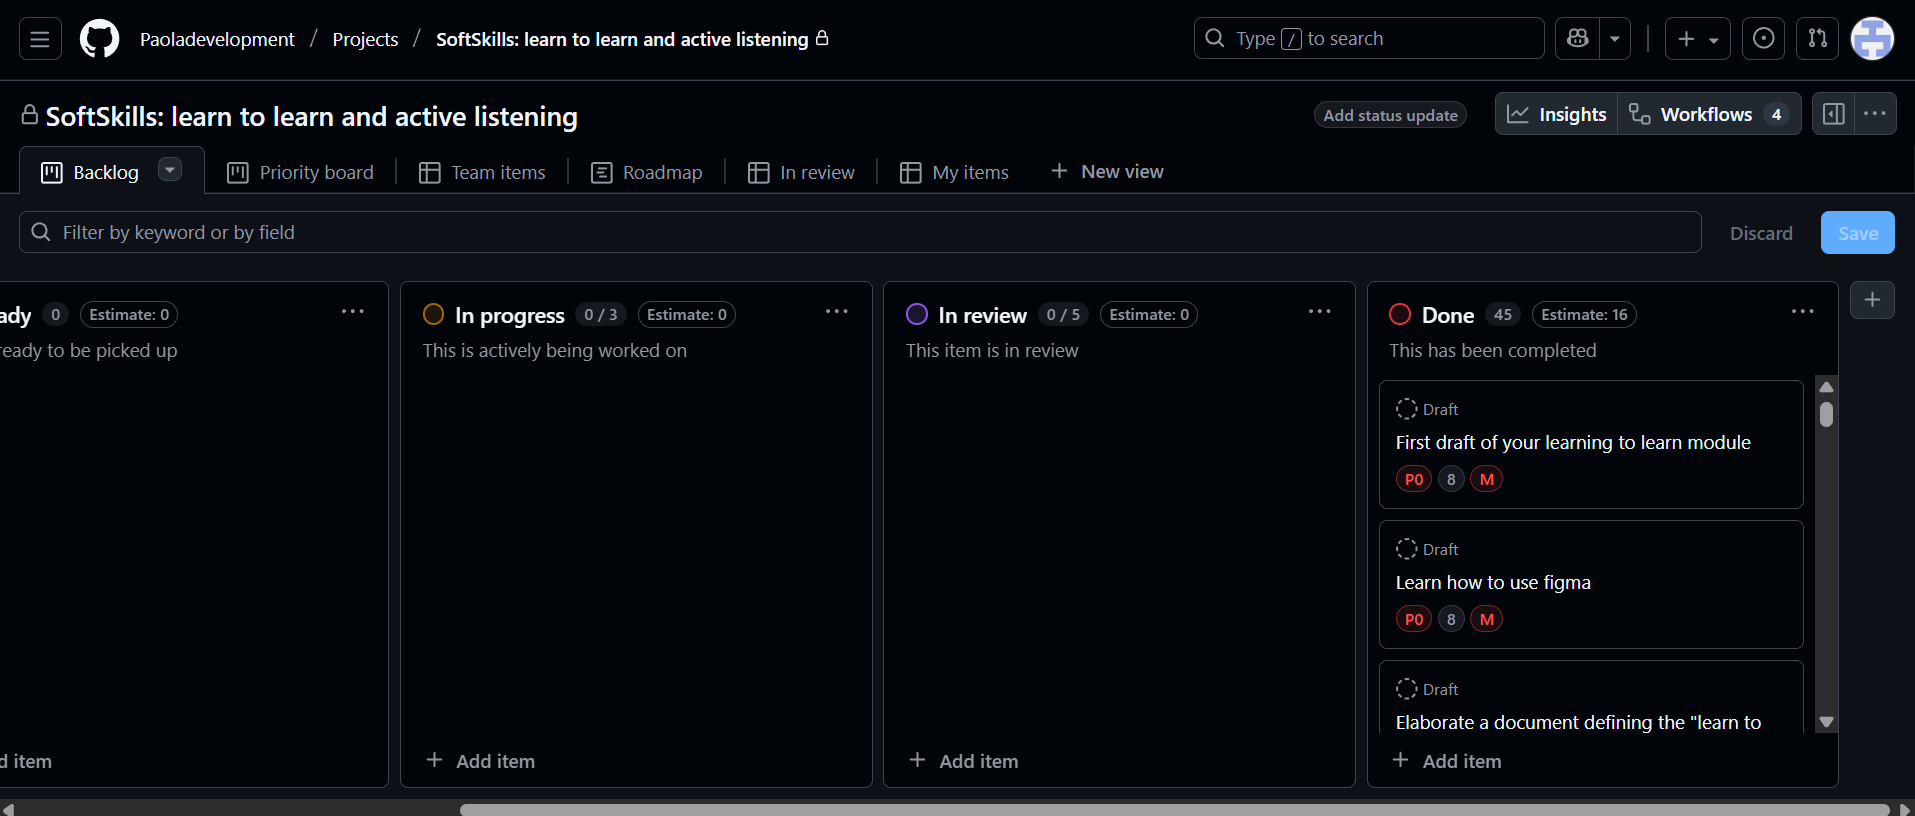
\includegraphics[width=\textwidth]{Figuras/tablero_github_projects.png}
\caption{Tablero Kanban del proyecto implementado en GitHub Projects.}
\label{fig:tablero_github}
\end{figure}

\subsection{Fase de definición y planificación inicial}

\begin{itemize}
    \item \textbf{Se definieron los objetivos del proyecto:}
    \begin{itemize}
        \item Se establecieron los objetivos generales y específicos.
        \item Se identificaron los entregables principales y los resultados esperados.
    \end{itemize}

    \item \textbf{Se creó el backlog inicial del proyecto:}
    \begin{itemize}
        \item Se listaron todas las tareas necesarias para desarrollar los módulos del sistema.
        \item Se priorizaron las tareas según su urgencia e impacto en el proyecto.
    \end{itemize}
\end{itemize}

\subsection{Fase de preparación y análisis de requisitos}

\begin{itemize}
    \item \textbf{Se recopilaron los requisitos del sistema:}
    \begin{itemize}
        \item Se realizaron sesiones de análisis para identificar y documentar los requisitos funcionales y no funcionales relacionados con los módulos de aprendizaje y escucha activa.
    \end{itemize}

    \item \textbf{Se analizaron, refinaron y validaron los requisitos:}
    \begin{itemize}
        \item Se detallaron, aclararon y reorganizaron los requisitos para asegurar su correcta comprensión y viabilidad técnica.
    \end{itemize}

    \item \textbf{Se actualizó el backlog:}
    \begin{itemize}
        \item Se añadieron nuevas tareas relacionadas con los requisitos identificados, incorporando refinamientos según su complejidad o dependencia.
    \end{itemize}
\end{itemize}

\subsection{Fase de diseño}

\begin{itemize}
    \item \textbf{Se diseñó la arquitectura del sistema:}
    \begin{itemize}
        \item Se elaboraron diagramas de la estructura general, se definieron los componentes principales del sistema y se establecieron las interacciones entre ellos.
    \end{itemize}

    \item \textbf{Se diseñó la interfaz de usuario:}
    \begin{itemize}
        \item Se desarrollaron prototipos de la interfaz del módulo Aprender a Aprender y del módulo de entrenamiento de escucha activa, definiendo elementos visuales y la experiencia de usuario (UX).
    \end{itemize}
\end{itemize}

\subsection{Fase de implementación}

\begin{itemize}
    \item \textbf{Se desarrollaron los módulos interactivos:}
    \begin{itemize}
        \item Se programaron las funcionalidades del sistema, incluyendo el módulo de gestión del aprendizaje, el editor de roadmaps y el módulo gamificado de escucha activa.
    \end{itemize}

    \item \textbf{Se integraron los componentes:}
    \begin{itemize}
        \item Se implementaron los diferentes elementos del backend y frontend, asegurando su correcto funcionamiento en conjunto y validando la comunicación entre los componentes.
    \end{itemize}

    \item \textbf{Se gestionó el trabajo con Scrumban:}
    \begin{itemize}
        \item El backlog se refinó continuamente y se utilizó el tablero Kanban para mover las tareas a través de las columnas “Pendiente”, “En Progreso” y “Hecho”, garantizando un flujo constante de avance.
    \end{itemize}
\end{itemize}

\subsection{Fase de pruebas}

\begin{itemize}
    \item \textbf{Se realizaron pruebas de usuario:}
    \begin{itemize}
        \item Se permitió que usuarios del sistema interactuaran con la plataforma, recopilando sus comentarios para identificar oportunidades de mejora que podrán incorporarse en futuras iteraciones.
    \end{itemize}
\end{itemize}